%
% This is the LaTeX template file for lecture notes for EE 382C/EE 361C.
%
% To familiarize yourself with this template, the body contains
% some examples of its use.  Look them over.  Then you can
% run LaTeX on this file.  After you have LaTeXed this file then
% you can look over the result either by printing it out with
% dvips or using xdvi.
%
% This template is based on the template for Prof. Sinclair's CS 270.

\documentclass[twoside]{article}
\usepackage{graphics}
\usepackage{xcolor}
\setlength{\oddsidemargin}{0.25 in}
\setlength{\evensidemargin}{-0.25 in}
\setlength{\topmargin}{-0.6 in}
\setlength{\textwidth}{6.5 in}
\setlength{\textheight}{8.5 in}
\setlength{\headsep}{0.75 in}
\setlength{\parindent}{0 in}
\setlength{\parskip}{0.1 in}

%
% The following commands set up the lecnum (lecture number)
% counter and make various numbering schemes work relative
% to the lecture number.
%
\newcounter{lecnum}
\renewcommand{\thepage}{\thelecnum-\arabic{page}}
\renewcommand{\thesection}{\thelecnum.\arabic{section}}
\renewcommand{\theequation}{\thelecnum.\arabic{equation}}
\renewcommand{\thefigure}{\thelecnum.\arabic{figure}}
\renewcommand{\thetable}{\thelecnum.\arabic{table}}

%
% The following macro is used to generate the header.
%
\newcommand{\lecture}[4]{
   \pagestyle{myheadings}
   \thispagestyle{plain}
   \newpage
   \setcounter{lecnum}{#1}
   \setcounter{page}{1}
   \noindent
   \begin{center}
   \framebox{
      \vbox{\vspace{2mm}
    \hbox to 6.28in { {\bf EE 382V: Social Computing
                        \hfill Fall 2018} }
       \vspace{4mm}
       \hbox to 6.28in { {\Large \hfill Lecture #1: #2  \hfill} }
       \vspace{2mm}
       \hbox to 6.28in { {\it Lecturer: #3 \hfill Scribe: #4} }
      \vspace{2mm}}
   }
   \end{center}
   \markboth{Lecture #1: #2}{Lecture #1: #2}
   %{\bf Disclaimer}: {\it These notes have not been subjected to the
   %usual scrutiny reserved for formal publications.  They may be distributed
   %outside this class only with the permission of the Instructor.}
   \vspace*{4mm}
}

%
% Convention for citations is authors' initials followed by the year.
% For example, to cite a paper by Leighton and Maggs you would type
% \cite{LM89}, and to cite a paper by Strassen you would type \cite{S69}.
% (To avoid bibliography problems, for now we redefine the \cite command.)
% Also commands that create a suitable format for the reference list.
\renewcommand{\cite}[1]{[#1]}
\def\beginrefs{\begin{list}%
        {[\arabic{equation}]}{\usecounter{equation}
         \setlength{\leftmargin}{2.0truecm}\setlength{\labelsep}{0.4truecm}%
         \setlength{\labelwidth}{1.6truecm}}}
\def\endrefs{\end{list}}
\def\bibentry#1{\item[\hbox{[#1]}]}

%Use this command for a figure; it puts a figure in wherever you want it.
%usage: \fig{NUMBER}{SPACE-IN-INCHES}{CAPTION}
\newcommand{\fig}[3]{
			\vspace{#2}
			\begin{center}
			Figure \thelecnum.#1:~#3
			\end{center}
	}
% Use these for theorems, lemmas, proofs, etc.
\newtheorem{theorem}{Theorem}[lecnum]
\newtheorem{lemma}[theorem]{Lemma}
\newtheorem{proposition}[theorem]{Proposition}
\newtheorem{claim}[theorem]{Claim}
\newtheorem{corollary}[theorem]{Corollary}
\newtheorem{definition}[theorem]{Definition}
\newenvironment{proof}{{\bf Proof:}}{\hfill\rule{2mm}{2mm}}

% **** IF YOU WANT TO DEFINE ADDITIONAL MACROS FOR YOURSELF, PUT THEM HERE:

\begin{document}
%FILL IN THE RIGHT INFO.
%\lecture{**LECTURE-NUMBER**}{**DATE**}{**LECTURER**}{**SCRIBE**}
\lecture{18}{October 27}{Vijay Garg}{Lydia Guarino}
%\footnotetext{These notes are partially based on those of Nigel Mansell.}

% **** YOUR NOTES GO HERE:

% Some general latex examples and examples making use of the
% macros follow.  
%**** IN GENERAL, BE BRIEF. LONG SCRIBE NOTES, NO MATTER HOW WELL WRITTEN,
%**** ARE NEVER READ BY ANYBODY.
\section{Pareto Dominant Strategies}
In a multi-participant game, one strategy profile is \emph{Pareto dominant} compared to another if it leaves at least one participant better off and no-one worse off.

\subsection{Definition}
Strategy profile $(s_1, s_2, ...s_n)$ \emph{Pareto dominates} strategy profile $(s_1^{'}, s_2^{'}, ...s_n^{'})$ iff:

$\forall i \in N: U_i(s_1, s_2, ...s_n) \geq U_i (s_1^{'}, s_2^{'}, ...s_n^{'})$ 

and

$\exists j \in N: U_j(s_1, s_2, ...s_n) > U_j (s_1^{'}, s_2^{'}, ...s_n^{'})$

\subsection{Example}
In the game represented below, strategy pair ($A_1$, $A_1$) Pareto dominates ($A_1$, $A_2$), because both players receive a higher payoff. ($A_2$, $A_1$) Pareto dominates ($A_2$, $A_2$) because Player 2 receives the same payoff as in ($A_2$, $A_2$), but Player 1 receives a higher payoff. ($A_1$, $A_2$) Pareto dominates ($A_2$, $A_2$) because Player 1 receives the same payoff, but Player 2 receives a higher payoff. ($A_2$, $A_2$) is Pareto dominated by all other strategies.

\begin{left}
\begin{tabular}{|c|c|c|}
\hline
x & $A_1$ & $A_2$\\
\hline
$A_1$ & 3, 5 & 2, 4\\
\hline
$A_2$ & 7, 2 & 2, 2\\
\hline
\end{tabular}
\end{left}

\section{Pareto Optimal Strategies}
Strategy profile $(s_1, s_2, ...s_n)$ is \emph{Pareto optimal} if there does not exist any strategy profile that \emph{Pareto dominates} $(s_1, s_2, ...s_n)$.

\subsection{Example}
In our same game, strategy pairs ($A_1$, $A_1$) and ($A_2$, $A_1$) are Pareto optimal because no other pair Pareto dominates them. 

\begin{left}
\begin{tabular}{|c|c|c|}
\hline
x & $A_1$ & $A_2$\\
\hline
$A_1$ & \colorbox{pink}{3, 5} & 2, 4\\
\hline
$A_2$ & \colorbox{pink}{7, 2} & 2, 2\\
\hline
\end{tabular}
\end{left}

\subsection{Poset example}

This same game can be represented as a poset, where it is immediately evident that these strategy pairs represent the maximal elements in the poset. Note that representative payoffs (3, 5) and (7, 2) are incomparable, which allows this game to have multiple Pareto optimal strategy profiles.

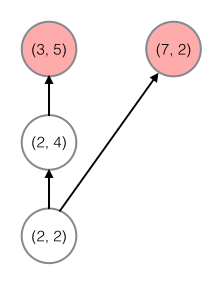
\includegraphics{poset.png}

\section{Pareto Optimality, Nash Equilibrium and Strictly Dominant Strategies}
Some interesting relationships to note for Pareto optimality are that strategy profiles that are Pareto optimal, may not be Nash Equilibrium or Strictly Dominant Strategies. In our example game of the Prisoner's Dilemma, you can see that the Nash Equilibrium and Strictly Dominant Strategy are for both suspects to confess, however, all strategy profiles \emph{except} a double confession are considered Pareto optimal.

\begin{left}
\begin{tabular}{|c|c|c|}
\hline
x & don't confess & confess\\
\hline
don't confess & \colorbox{pink}{-1, -1} & \colorbox{pink}{-10, 0}\\
\hline
confess & \colorbox{pink}{0, -10} & -4, -4\\
\hline
\end{tabular}
\end{left}

\section{Social Optimality}
Strategy profile $(s_1, s_2, ...s_n)$ is \emph{Socially optimal } if the sum of the payoffs in the strategy are maximized for the choice.

\begin{lemma}
Social optimality implies Pareto optimality.
\end{lemma}

\begin{left}
\begin{tabular}{|c|c|c|}
\hline
x & $A_1$ & $A_2$\\
\hline
$A_1$ & 3 + 5 = 8 & 2 + 4 = 6\\
\hline
$A_2$ & \colorbox{pink}{7 + 2 = 9} & 2 + 2 = 4\\
\hline
\end{tabular}
\end{left}

\end{document}





